\subsection{Load Snapshot Sequenzdiagramm}

Das obige Diagramm zeigt die Speicherroutine der Commands und Snapshots des Graphen. Beim Start des ReplayLogSaveService erstellt sich dieser einen Replay-, Command- und Snapshotlogger, um sich später einen ReplayLog zusammenzustellen. Der ReplayLogSaveService ist ein Listener beim TruffleReceiver. Dadurch können die eingehenden Commands im CommandLogger gespeichert werden. Jeweils nach einem bestimmten Zeitintervall in der Endlosschleife wird ein Snapshot von dem Graphen erstellt und zusammen mit den gesammelten Commands in einem ReplayLog serialisiert.

\begin{sidewaysfigure}
  \centering
  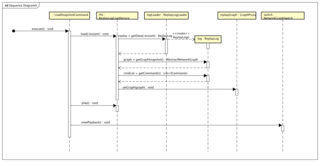
\includegraphics[width=\textwidth]{../diagramimages/sd_loadsnapshot.png}
  \caption[Sequenzdiagramm Load Snapshot Sequenzdiagramm]{Sequenzdiagramm Load Snapshot Sequenzdiagramm}
\end{sidewaysfigure}
\FloatBarrier
